\section{The Large Hadron Collider at CERN}%
\label{sec:lhc}

In this chapter, the ATLAS experiment at the Large Hadron Collider (LHC) of
CERN\footnote{From the French \emph{Conseil Européen pour la Recherche
    Nucléaire} referring to both the research organisation and the laboratory
  located in Geneva, Switzerland.} is introduced. The LHC is the world's
highest-energy, laboratory-based particle collider experiment, which allows to
study the direct production of Higgs boson pairs with unprecedented precision.
Particle collision events are recorded and reconstructed using the ATLAS
detector, which is one of two general-purpose particle detector experiments at
the LHC.

Centre of mass energy and instantaneous / integrated luminosity.

% - Energy to produce Higgs boson pairs can, at present, not be achieved with
%   electron positron colliders -> VHH production which would require CMS in excess of 300 GeV

% - Cross section of HH production - Ndot = L * sig
% - LHC proton and heavy-ion collider, though exclusively working with \pp
% collision data.
% -

CERN

\begin{figure}[htbp]
  \centering

  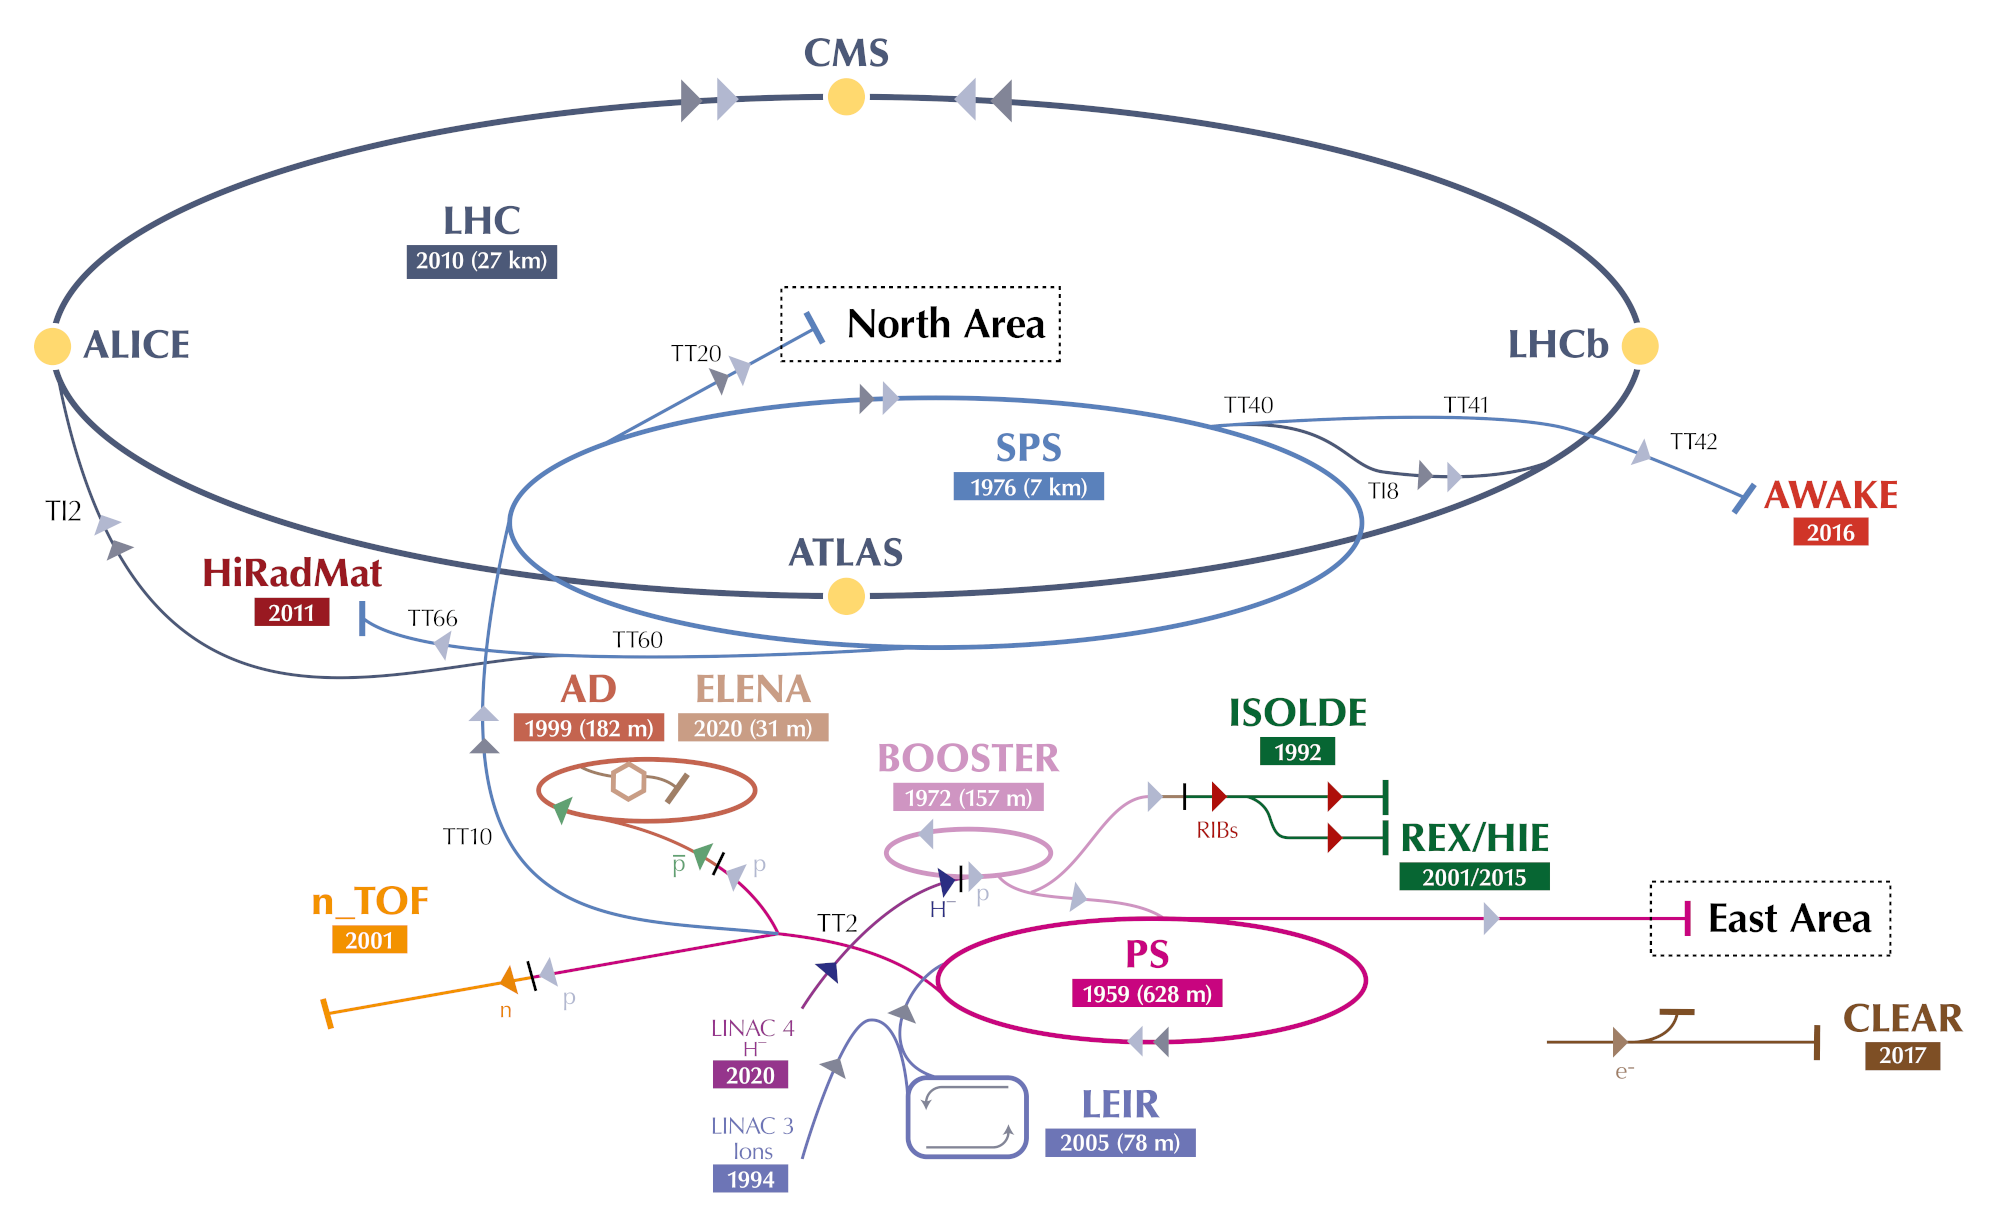
\includegraphics[width=0.9\textwidth, trim=10.5cm 44cm 2cm 20cm,
  clip]{lhc/cern_complex}

  \caption{The CERN accelerator complex in August 2018. Image adapted from
    Ref.~\cite{Mobs:2684277}.}%
  \label{fig:bla}
\end{figure}

Notes:
\begin{itemize}

\item Large Hadron Collider~\cite{Evans:2008zzb}: Geneva, Switzerland / European
  complex of the Organization for Nuclear Research, CERN, ...

  greater Geneva area close to the French--Swiss border

\item Proton \& Heavy Ion Collider; ca.\ \SI{26.7}{\kilo\metre} circumference
  (underground) built into the former LEP tunnel
  \begin{itemize}

  \item Synchrotron: 1232 dipoles (superconducting) -> Magnetic field of
    \SI{8.3}{\tesla} required for \SI{7}{\TeV} beam energy operation /
    quadrupole magnets for focussing of the beam

  \item Two proton beams circulating in opposite directions. In bunches. What
    are bunches? -> Symmetric

  \item Accelerator chain (\pp): LINAC 2 (\textbf{LIN}ear \textbf{AC}celerator)
    -> Proton Synchrotron Booster -> Proton Synchrotron (PS) -> Super Proton
    Synchrotron (SPS) (injection energy of \SI{450}{\GeV})-> LHC
  \end{itemize}

\item Provides high-energy particle collisions for four large scale experiments:
  ATLAS, CMS~\cite{CMS-CMS-00-001}, ALICE~\cite{ALICE:2008ngc}, and
  LHCb~\cite{LHCb:2008vvz}; Smaller experiments?  MOEDAL~\cite{MoEDAL:2009jwa},
  TOTEM~\cite{TOTEM:2008lue}

\item What is the goal of the LHC? -> energy frontier (protons instead of
  electrons due to reduced synchrotron radiation)

\item Run history (time?): Run 1 \SI{7}{\TeV} (2009--2011) / \SI{8}{\TeV}
  (2012); Run 2 \SI{13}{\TeV} (2015--2018); Run 3 \SI{13.6}{\TeV} (2022--)
  commenced in 2022 and, at present, is forseen to end in 2026.

\item Performance characteristics of the \pp operation of the LHC during Run~2:

  \begin{itemize}
  \item Bunches \& Bunch spacing: 2556 (\SI{25}{\nano\second}) -- but 2808 RF
    buckets (not all filled)
  \item Protons per bunch: \num{1.1e11}
  \item Luminosity: \SI{2.1e34}{\per\centi\metre\squared\per\second} (design:
    \SI{1.0e34}{\per\centi\metre\squared\per\second})
  \item $\sqrt{s} = \SI{13}{\TeV}$
  \item Pile-up?
  \item Delivered integrated luminosity: about \SI{160}{\ifb}
    \end{itemize}

\item How is the luminosity of a collider calculated?

\item How does Luminosity relate to event rate / pile-up?
  \begin{align*}
    \frac{\mathrm{d}N}{\mathrm{d}t} = L \sigma
  \end{align*}
  Inelastic \pp cross-section at $\sqrt{s} = \SI{13}{\TeV}$ ca.\
  \SI{80}{\milli\barn}~\cite{STDM-2015-05}.

\end{itemize}

% Luminosity or pile-up plots?
% https://twiki.cern.ch/twiki/bin/view/AtlasPublic/LuminosityPublicResultsRun2

\begin{figure}[htbp]
  \centering

  \begin{subfigure}{0.47\textwidth}
    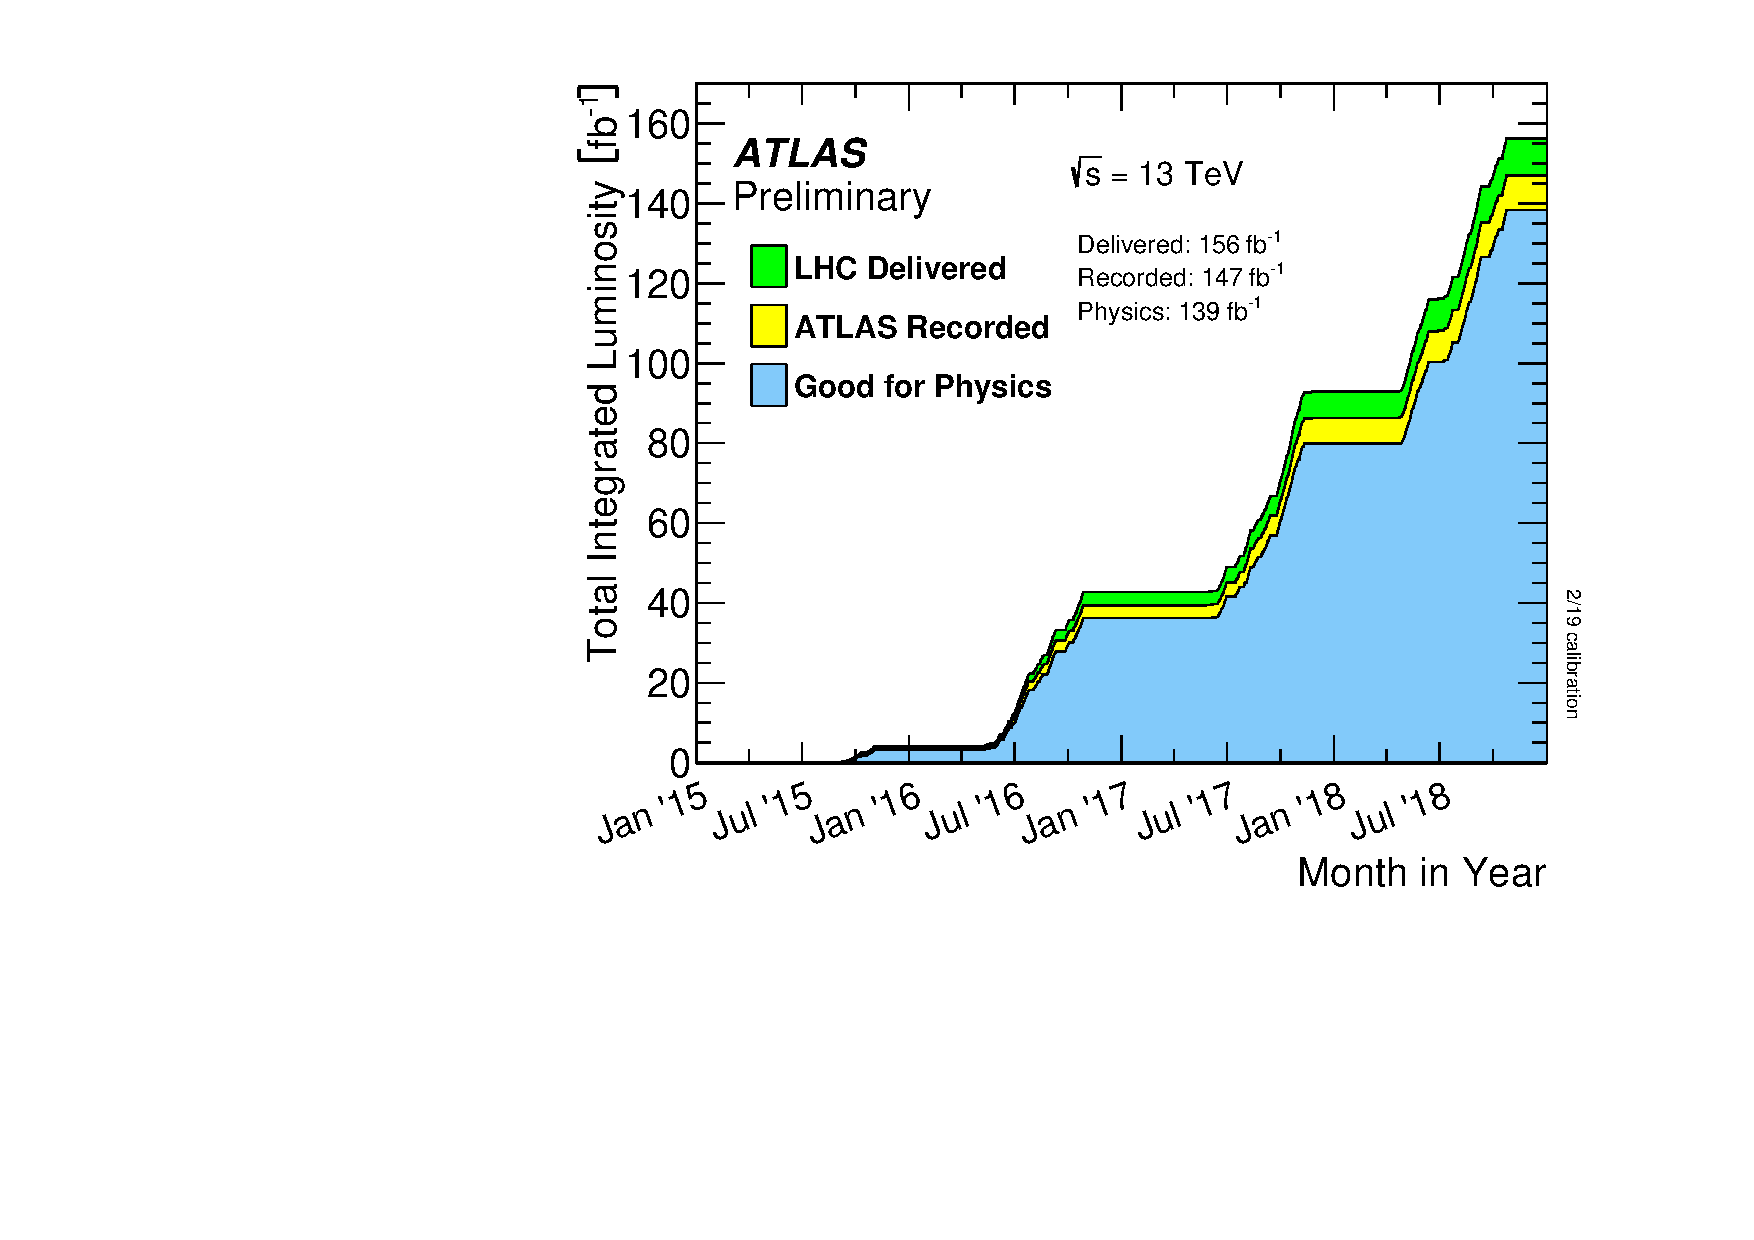
\includegraphics[width=\textwidth]{lhc/int_lumi_vs_time}
    \subcaption{}
  \end{subfigure}\hspace*{0.02\textwidth}%
  \begin{subfigure}{0.47\textwidth}
    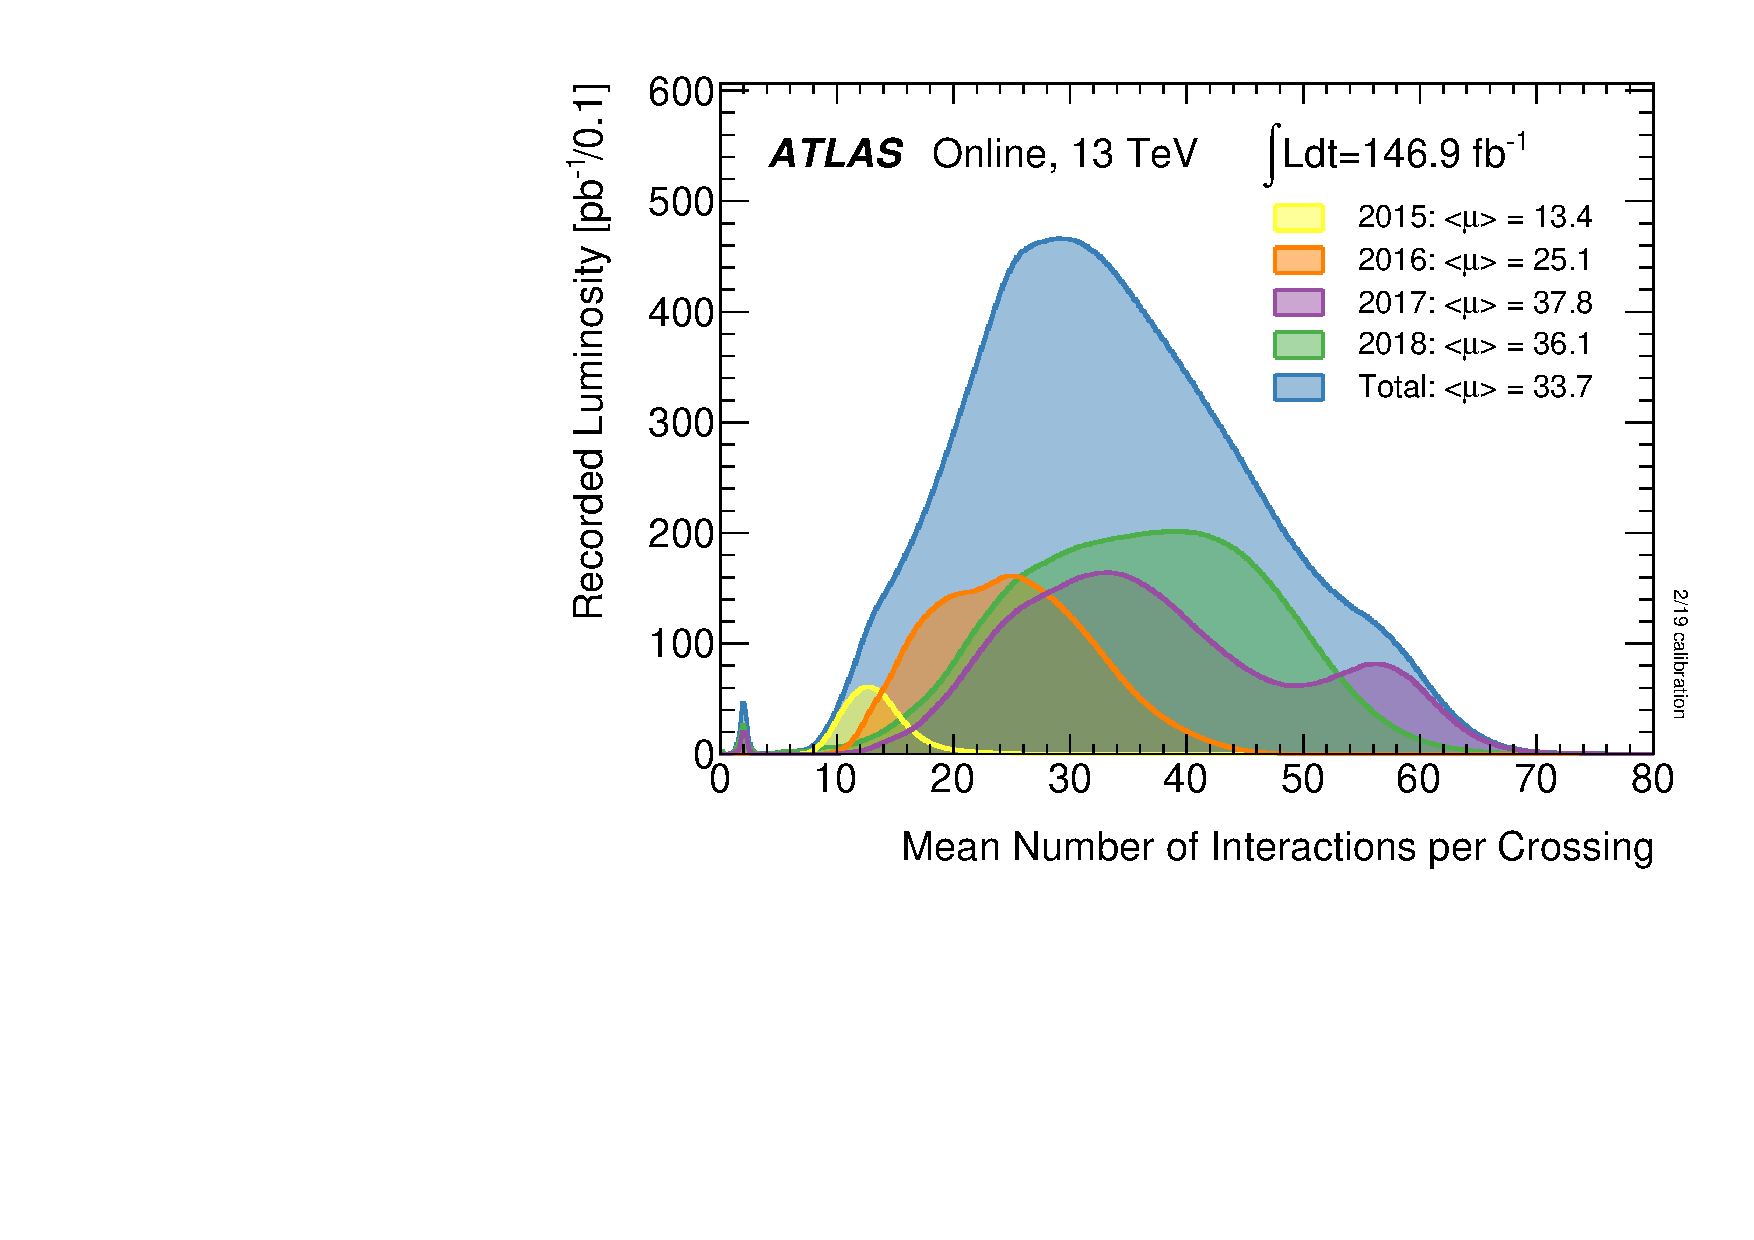
\includegraphics[width=\textwidth]{lhc/mu_2015_2018}
    \subcaption{}
  \end{subfigure}

  \caption{The integrated luminosity as a function of time (a) and the
    luminosity-weighted mean number of interactions per bunch-crossing (b) of
    LHC in \pp operation mode during Run~2. In figure (a), the integrated
    luminosity delivered by the LHC (green), recorded by the ATLAS detector
    (yellow), and the integrated luminosity of the \pp-collision dataset passing
    the data-qualtiy criteria~\cite{DAPR-2018-01} of the ATLAS collaboration
    (blue) is shown. The mean number of interactions per bunch-crossing, $\mu$,
    is calculated from the instantaneous luminosity assuming an inelastic \pp
    cross-section at $\sqrt{s} = \SI{13}{\TeV}$ of \SI{80}{\milli\barn}. The
    figures are taken from~\cite{atlas_luminosity_summary_plots}.}%
  \label{fig:lumi_and_pu}
\end{figure}

%%% Local Variables:
%%% mode: latex
%%% TeX-master: "../../phd_thesis"
%%% End:
